%! Author = user
%! Date = 3/9/2024

% Preamble
\documentclass{article}
\usepackage[utf8]{inputenc}
\usepackage{amsmath, amssymb, amsthm}
\usepackage{tikz}
\usepackage{pgfplots}
\usepackage{subfigure}

\title{LaTex for Students}
\author{Jun Ho Lee}
\date{March 2024}

% Document
\begin{document}

\newpage

\section{Week1}

Introduction to Deep Learning.

\subsection{What is a Neural Network?}

\subsection{Supervised Learning with Neural Networks}

\subsection{Why is Deep Learning taking off?}

\subsection{About this Course}
    \begin{enumerate}
        \item Neural Networks and Deep Learning
        \item Improving Deep Neural Networks: Hyperparameter  tuning, Regularization and Optimization
        \item Structuring your Machine Learning project
        \item Convolutional NeuralNetworks
        \item Natural Language Processing: Building sequence models
    \end{enumerate}

\subsection{Outline of this Course}
    \begin{itemize}
        \item{Week1. Introduction}
        \item{Week2. Basics of Neural Network programming}
        \item{Week3. One hidden layer Neural Networks}
        \item{Week4. Deep Neural Networks}
    \end{itemize}


\newpage

\section{Week2}

Basics of Neural Network Programming

How do I write an equation in \LaTeX?\\

\begin{center}
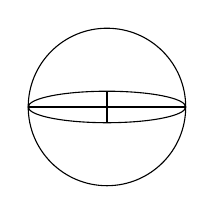
\begin{tikzpicture}
    \centering
    \draw (0,0) ellipse (1cm and 0.2cm);
    \draw (0,0) circle (1cm);
    \draw (0,-0.2) -- (0,0.2);
    \draw (-1,0) -- (1,0);
\end{tikzpicture}
\end{center}

In 1902, Einstein created this equation: $E=mc^2$

And Newton came up with this one: $\sum F=ma$

\begin{equation}
    5+5=10
\end{equation}

\begin{equation}
    \begin{split}
        A & = \frac{5\pi r^2}{2} \\
        A & = \frac{1}{2} \pi r^2
    \end{split}
\end{equation}

\newpage

\subsection{Neural Network Notations}

\textbf{General comments:}\\
superscript $(i)$ will denote the $i^{th}$ training example. \\
superscript $[l]$ will denote the $l^{th}$ layer.\\

\textbf{Sizes:}
\begin{itemize}
    \item[-]{m: number of examples in the dataset}
    \item[-]{$n_x$: input size}
    \item[-]{$n_y$: output size}
    \item[-]{$n_h^{[l]}$: number of hidden units of the ${l^th}$ layer. \\ In a for loop, it is possible to denote $n_x = n_h^{[0]}$ and $n_y = n_h^{[number of layer+1]}$ }
    \item[-]{$L$: number of layers in the network}
\end{itemize}

\textbf{Objects:}
\begin{itemize}
    \item[-]{$X \in \mathbb{R}^{n_x \times m}$ is the input matrix}
    \item[-]{$x^{(i)} \in \mathbb{R}^{n_x} is the i^{th} example represented as a column vector $}
    \item[-]{$Y \in \mathbb{R}^{n_y \times m}$ is the label matrix}
    \item[-]{$y^{(i)} \in \mathbb{R}^{n_y}$ is the output label for the $i^{th}$ example}
    \item[-]{$W^{[l]} \in \mathbb{R}^{number of units in next layer \times number of units in the previous layer}$ is the weight matrix, superscript $[l]$ indicates the layer}
    \item[-]{}
\end{itemize}

\textbf{Common forward propagation equation examples:}
\begin{itemize}
    \item[-]{}
    \item[-]{}
\end{itemize}

\textbf{Examples of cost functions:}
\begin{itemize}
    \item[-]{}
    \item[-]{}
\end{itemize}

\newpage

\subsection{Binary Classification}

Use matrix without using for loops.\\
Computation using Forward propagation and Backward propagation.\\
Logistic regression is an algorithm for binary classification.\\

m training examples
$\{(x^{(1)}, y^{(1)}), (x^{(2)}, y^{(2)}), \hdots, (x^{(m)}, y^{(m)})\}$ \\
where $x^{(i)} \in \mathbb{R}^{n_x}$ and $y^{(i)} \in \{0,1\}$ for $i \in [1,m]$ \\

$X =
\begin{bmatrix}
    \vdots & \vdots & \vdots \\
    X^{(1)} & X^{(1)} & X^{(m)} \\
    \vdots & \vdots & \vdots \\
\end{bmatrix}
\in \mathbb{R}^{n_x \times m}
$\\

$X.shape = (n_x, m)$\\

$Y = [Y^{(1)}, Y^{(2)}, \hdots, Y^{(m)}]
\in \mathbb{R}^{1 \times m}
$\\

$Y.shape = (1, m)$\\

\newpage
\subsection{Logistic Regression}

Given $X$, want $\hat{Y} = P(Y=1 |X)$ where $X \in \mathbb{R}^{n_x}$\\

    Parameters: $\omega \in \mathbb{R}^{n_x}$ a $n_x$ dimensional vector, $b \in \mathbb{R}$ a real number.\\

    Output $\hat{y} = \sigma(\omega^{T}X + b) = \sigma(z)$\\

$\displaystyle \sigma (z)=\frac {1}{1+e^{-z}}$\\

Drawing a sigmoid function and its derivative in tikz\\

\pgfplotsset{compat=1.16}
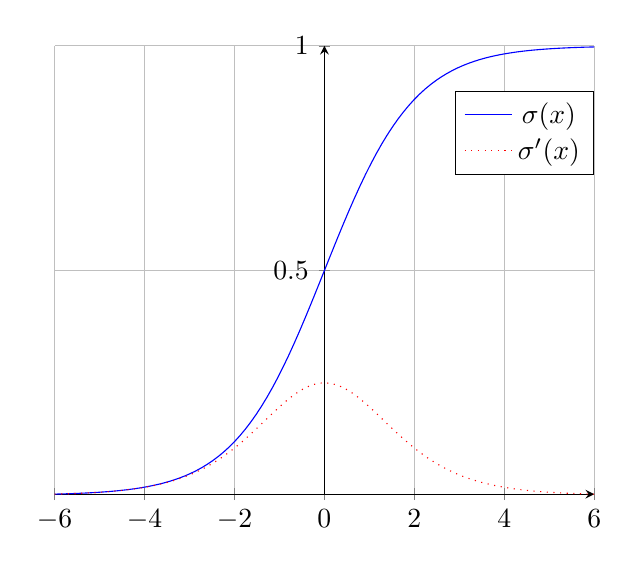
\begin{tikzpicture}[declare function={sigma(\x)=1/(1+exp(-\x));
sigmap(\x)=sigma(\x)*(1-sigma(\x));}]
\begin{axis}%
[
    grid=major,
    xmin=-6,
    xmax=6,
    axis x line=bottom,
    ytick={0,.5,1},
    ymax=1,
    axis y line=middle,
    samples=100,
    domain=-6:6,
    legend style={at={(1,0.9)}}
]
    \addplot[blue,mark=none]   (x,{sigma(x)});
    \addplot[red,dotted,mark=none]   (x,{sigmap(x)});
    \legend{$\sigma(x)$,$\sigma'(x)$}
\end{axis}
\end{tikzpicture}


\newpage
\subsection{Logistic Regression Cost Function}

To train the parameter $\omega$ and $b$ of a Logistic Regression Model, we need a cost function.\\

    $\hat{y} = \sigma{(\omega^{T}X + b)}$ where $\sigma(z) = \frac{1}{1+e^{-z}}$\\

    $\hat{y}^{(i)} = \sigma{(\omega^{T}X^{(i)} + b)}$ where $\sigma(z^{(i)}) = \frac{1}{1+e^{{-z}^{(i)}}}$\\

    Given $\{(x^{(1)}, y^{(1)}), (x^{(2)}, y^{(2)}), \hdots, (x^{(m)}, y^{(m)})\}$, want $\hat{y}^{(i)} \approx y^{(i)}$. \\

    Loss(error) function (for a single training Example):

    $\displaystyle \mathcal{L}(\hat{y}, y) = -(y\log{\hat{y}} + (1-y)\log{(1-\hat{y}))}$\\

    Cost function (for the entire training Examples):

    $\displaystyle \mathcal{J}(\omega, b) = \frac{1}{m}\sum_{i=1}^{m} \mathcal{L}(\hat{y}^{(i)}, y^{(i)}) = -\frac{1}{m}\sum_{i=1}^{m} [y^{(i)}\log{\hat{y}^{(i)}} + (1-y^{(i)})\log{(1-\hat{y}^{(i)})}]$\\\\

    The loss function computes the error for a single training example; the cost function is the average of the loss functions of the entire training set.\\

    In training logistic regression model, we will try to find $\omega$ and $b$ such that they minimize the Cost function $\mathcal{J}(\omega, b)$.\\

    Logistic Regression can be seen as a very small Neural Network.\\


\newpage
\subsection{Gradient Descent}

$\displaystyle \mathcal{J}(\omega, b) = \frac{1}{m}\sum_{i=1}^{m} \mathcal{L}(\hat{y}^{(i)}, y^{(i)}) = -\frac{1}{m}\sum_{i=1}^{m} [y^{(i)}\log{\hat{y}^{(i)}} + (1-y^{(i)})\log{(1-\hat{y}^{(i)})}]$\\\\

    Want to find $\omega$ and $b$ that minimize the Cost function $\mathcal{J}(\omega,b)$.

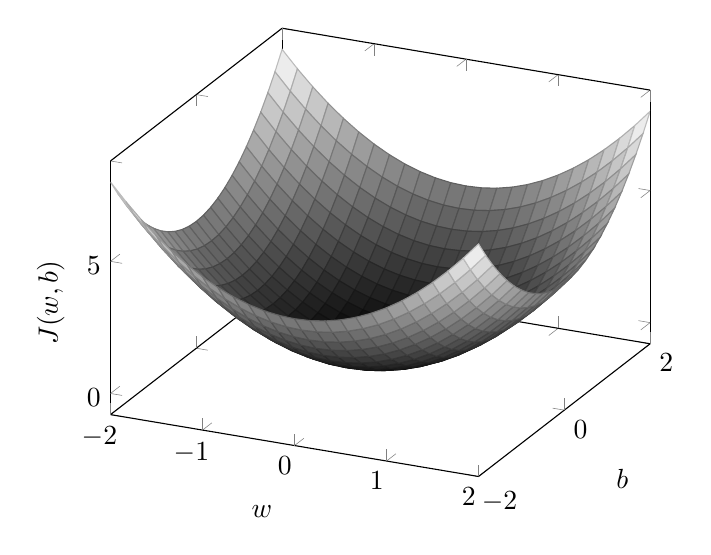
\begin{tikzpicture}
\begin{axis}[
    xlabel=$w$,
    ylabel=$b$,
    zlabel={$J(w,b)$}
]
\addplot3[surf,domain=-2:2, colormap/blackwhite] {x^2+y^2};
\end{axis}
\end{tikzpicture}\\

    $\mathcal{J}(\omega,b)$ is a convex function with a single local optimum.\\
    No matter where you initialize the point, you should get to the same point (Global optimum).\\

    Repeat: \\

        $\omega := \omega - \alpha \frac{\partial\mathcal{J}(\omega,b)}{\partial\omega}$\\

        $\omega := \omega - \alpha d\omega$\\

        $b := b - \alpha \frac{\partial\mathcal{J}(\omega,b)}{\partial b}$\\

        $b := b - \alpha db$\\

        where $\alpha$ is the learning rate.\\

\end{document}

